\documentclass[11pt, a4paper]{article}
\usepackage[margin=2.2cm]{geometry}
\usepackage[T1]{fontenc}
\usepackage{lmodern}          % Type 1 vector fonts
\usepackage{cmap}             % ToUnicode CMap -> copyable text and accents
\usepackage[utf8]{inputenc}
\usepackage[english]{babel}
\usepackage{amsmath, amssymb}
\usepackage{icomma}           % decimal comma, as in the instructor's keys
\usepackage{enumitem}
\usepackage{xcolor}
\usepackage{graphicx}
\usepackage{parskip}
\usepackage{needspace}
\usepackage{hyperref}
\usepackage{fancyhdr}

\definecolor{hl}{gray}{0.84}
\definecolor{margem}{gray}{0.45}
\hypersetup{colorlinks=true, linkcolor=black, urlcolor=black,
  pdftitle={PSET 7 --- short solution --- Macroeconomics I MPE Insper}}

\pagestyle{fancy}
\fancyhf{}
\renewcommand{\headrulewidth}{0pt}
\fancyfoot[C]{\small\textcolor{margem}{PSET 7 --- short version --- \thepage}}

% The instructor's marks: a highlighted result, a margin warning, an item label.
\newcommand{\res}[1]{\colorbox{hl}{$\displaystyle #1$}}
\newcommand{\rest}[1]{\colorbox{hl}{#1}}
\newcommand{\nota}[1]{\par\hfill\textcolor{margem}{\small\itshape\#\,#1}\par}
\newcommand{\q}[1]{\par\medskip\needspace{4\baselineskip}\noindent\textbf{\large(#1)}\quad}
\newcommand{\itm}[1]{\par\smallskip\needspace{3\baselineskip}\noindent\textbf{(#1)}\quad}
\newcommand{\MRS}{\mathrm{MRS}}
\newcommand{\MRT}{\mathrm{MRT}}
\newcommand{\ra}{\;\rightarrow\;}
\newcommand{\Sg}{\left(\sigma^{-1}+\eta\right)}
\setlist{itemsep=1pt, topsep=2pt, leftmargin=1.3em}

\begin{document}

\noindent{\Large\bfseries PSET 7 --- short solution}\hfill
{\small Macro I --- MPE Insper --- Benigno (2015)}\\[-4pt]
\rule{\textwidth}{0.6pt}

{\small\textcolor{margem}{Same answers as \texttt{lista7\_resolucao.pdf}, in the format of the
instructor's keys: arrow chains instead of paragraphs, results highlighted, traps as \# notes.
Every step is shown. Lower-case letters are log-deviations from an efficient steady state.
Calibration (Benigno p.~515, fn.~24): $\alpha=0{,}66$, $\sigma=0{,}5$, $\eta=0{,}2$, $\theta=8$,
$\rho=2\%$. SR = short run, LR = long run.}}

\nota{Here $\sigma$ \emph{is} the EIS (scaled by $s_c=C/Y$: $\sigma=s_c\tilde\sigma$); in Kurlat
$\sigma$ is curvature and $1/\sigma$ the EIS. Opposite conventions.}

%=====================================================================
\q{1} NK vs New Classical (NC) vs original Keynesian (K)

\noindent\colorbox{hl}{\parbox{\dimexpr\linewidth-2\fboxsep}{\textbf{Summary:} NK = NC
method (optimisation, rational expectations) + K friction (prices don't clear in the SR),
plus monopolistic competition and an interest-rate instrument.}}

\itm{i} \textbf{Prices, expectations, monetary policy}
\begin{itemize}
\item K: rigidity assumed, adaptive/no expectations $\ra$ stable, exploitable Phillips
      curve $\ra$ money has lasting real effects.
\item NC: flexible prices, RE $\ra$ only surprises move $y$ (Lucas) $\ra$ systematic policy
      ineffective (Sargent--Wallace).
\item NK: RE + share $\alpha$ of firms keeps a price $p^e$ set \emph{before} the shock. The AS
      curve follows in four steps:
\end{itemize}
\begin{enumerate}[label=\arabic*., leftmargin=2.2em]
\item Adjusting firm: $\tilde P=(1+\mu)\dfrac{W}{A}\ra\dfrac{\tilde P}{P}=(1+\mu)\dfrac{W/P}{A}$;
      household: $\dfrac WP=\dfrac{v_l(L)}{u_c(C)}=L^{\eta}C^{\tilde\sigma^{-1}}$.
\item Flexible prices ($\tilde P=P$) define $Y_n$: $(1+\mu)\dfrac{L_n^{\eta}C_n^{\tilde\sigma^{-1}}}{A}=1$.
      Divide step 1 by this and take logs:
      $\tilde p-p=\eta(y-y_n)+\tilde\sigma^{-1}(c-c_n)$.
\item $y=s_c c+g\ra c-c_n=\dfrac{y-y_n}{s_c}$, and $\tilde\sigma^{-1}=s_c\sigma^{-1}$
      $\ra\tilde p-p=\Sg(y-y_n)$ \quad(real marginal cost).
\item Index: $p=\alpha p^e+(1-\alpha)\tilde p\ra\tilde p-p=\dfrac{p-\alpha p^e}{1-\alpha}-p
      =\dfrac{\alpha}{1-\alpha}(p-p^e)$. Equate with step 3:
\end{enumerate}
\[
\res{p-p^e=\kappa(y-y_n),\qquad \kappa=\frac{(1-\alpha)\Sg}{\alpha}}
\qquad \kappa=\frac{0{,}34\cdot2{,}2}{0{,}66}=\frac{0{,}748}{0{,}66}=1{,}133
\]
\begin{itemize}
\item Same equation as Lucas, but $p^e$ is a \emph{posted price}, not a forecast\\
      $\ra$ \rest{known policy reacting after $p^e$ is set still moves $y$}.\\
      LR: all firms reset $\ra y=\bar y_n$ (vertical LR AS) $\ra$ money neutral.
\item Evidence: 1970s stagflation (keep RE); announced disinflations still cost output
      (need a friction that fools no one); micro prices last $\approx3$ quarters
      $\ra\alpha\approx0{,}66$.
\item Implication: $\partial\kappa/\partial\alpha<0$ ($\alpha$ in the denominator)
      $\ra$ more rigidity $\ra$ flatter AS; $\alpha\to0\ra\kappa\to\infty\ra$ classical.
\end{itemize}
\nota{Same curve as Lucas (Benigno p.~508), not the forward-looking NKPC.}

\itm{ii} \textbf{Market structure}
\begin{itemize}
\item K: unmodelled / rigid nominal wage with competitive firms $\ra$ firms on falling $MPL$
      $\ra$ countercyclical real wage (not in data).
\item NC: perfect competition $\ra$ nobody sets a price $\ra$ nobody to be sticky.
\item NK: Dixit--Stiglitz demand $Y(j)=\left(\tfrac{P(j)}{P}\right)^{-\theta}(C+G)$, cost $\tfrac WA$ per unit.
      Profit $\Pi=P(j)^{1-\theta}P^{\theta}(C+G)-\tfrac WA P(j)^{-\theta}P^{\theta}(C+G)$.\\
      FOC: $(1-\theta)P(j)^{-\theta}+\theta\tfrac WA P(j)^{-\theta-1}=0$
      $\ra$ multiply by $P(j)^{\theta+1}$: $(\theta-1)P(j)=\theta\tfrac WA$
      $\ra\res{P(j)=\underbrace{\tfrac{\theta}{\theta-1}}_{\text{mark-up}}\tfrac WA}$ \;($\theta>1$).
\item Consequences: (1) firms \emph{set} prices; (2) $P>MC\ra$ a firm stuck at $p^e$ gains on
      each extra unit $\ra$ \rest{serves demand: $y$ demand-determined in the SR};
      (3) mark-up = wedge $\ra y_n<y_e$ (Q3).
\item Menu cost: firm's loss from not adjusting is 2nd order (envelope: $\partial\Pi/\partial P(j)=0$
      at the optimum); aggregate output effect is 1st order (Mankiw 1985).
\end{itemize}

\itm{iii} \textbf{Aggregate demand and the instrument}
\begin{itemize}
\item K: IS (consumption function) + LM (money demand); CB sets $M$; slope via real balances
      ($P\uparrow\ra M/P\downarrow\ra i\uparrow\ra I\downarrow$).
\item NC: $MV=PY$; $M$ is the instrument and the nominal shock.
\item NK: AD from the Euler equation, CB sets $i$, no LM. Derivation:
\end{itemize}
\begin{enumerate}[label=\arabic*., leftmargin=2.2em]
\item Euler: $u_c(C)=\beta(1+i)\dfrac{P}{\bar P}u_c(\bar C)$, with $u_c=C^{-\tilde\sigma^{-1}}$.
\item Logs ($\ln\beta=-\rho$, $\ln(1+i)\approx i$):
      $-\tilde\sigma^{-1}c=-\rho+i+p-\bar p-\tilde\sigma^{-1}\bar c$
      $\ra c=\bar c-\tilde\sigma\left[i-(\bar p-p)-\rho\right]$.
\item Multiply by $s_c$ and use $y-g=s_c c$, $\bar y-\bar g=s_c\bar c$, $\sigma=s_c\tilde\sigma$,
      $\bar y=\bar y_n$:
\end{enumerate}
\[
\res{y=\bar y_n+(g-\bar g)-\sigma\left[i-(\bar p-p)-\rho\right]}\qquad
\left.\frac{dp}{dy}\right|_{AD}=-\frac1\sigma<0
\]
\begin{itemize}
\item Slope: $p\uparrow\ra(\bar p-p)\downarrow$ (expected inflation) $\ra r=i-(\bar p-p)\uparrow
      \ra C\downarrow\ra y\downarrow$.
\item Evidence: CBs target short rates; money demand unstable. Implication: transmission via
      $r$; expectations ($\bar y_n$, $\bar p$) shift demand today; ZLB possible.
\end{itemize}
\nota{No LM curve: never explain AD's slope with money demand.}

\itm{iv} \textbf{Microfoundations and welfare}
\begin{itemize}
\item K: postulated equations, ad hoc loss. NC: micro-founded but competitive $\ra$ efficient
      (1st welfare theorem) $\ra$ nothing to stabilise.
\item NK: micro-founded \emph{with} distortions ($\mu$, sticky $p$) $\ra$ loss derived from
      utility (2nd-order approximation around the efficient SS, Benigno eq.~33, after
      Woodford 2003):\\[2pt]
      \res{L=\tfrac12(y-y_e)^2+\tfrac{\theta}{2\kappa}(p-p^e)^2}
\item Reading: target $y_e$ (not $y_n$); only surprises $p-p^e$ cost (dispersion between
      adjusters and frozen firms); weight $\tfrac\theta\kappa=\tfrac{\theta\alpha}{(1-\alpha)\Sg}$
      $\ra\uparrow$ in $\alpha$ and in $\theta$.
\item Evidence: Lucas critique (1970s model failures) $\ra$ deep parameters
      $(\beta,\tilde\sigma,\eta,\theta,\alpha)$.
\end{itemize}
\nota{The approximation itself is not derived in the article; the course takes eq.~33 as given.}

%=====================================================================
\q{2} AS--AD. Start $E$: $i=\rho$, $y=y_n=y_e=0$, $p=p^e=\bar p$, $g=\bar g$.

\textbf{Closed form} (used in both items). Put AS, $p=p^e+\kappa(y-y_n)$, into AD with $\bar p=p^e$:
\begin{align*}
y&=\bar y_n-\sigma\left[i-p^e+p^e+\kappa(y-y_n)-\rho\right]
  =\bar y_n-\sigma(i-\rho)-\sigma\kappa(y-y_n)\\
y-y_n&=(\bar y_n-y_n)-\sigma(i-\rho)-\sigma\kappa(y-y_n)\\
(1+\sigma\kappa)(y-y_n)&=\sigma\left[\underbrace{\rho+\sigma^{-1}(\bar y_n-y_n)}_{\equiv\, r_n}-i\right]
\end{align*}
\[
\res{y-y_n=\frac{\sigma}{1+\sigma\kappa}(r_n-i),\qquad p-p^e=\kappa(y-y_n)}
\qquad \sigma\kappa=0{,}5\cdot1{,}133=0{,}567,\;\;1+\sigma\kappa=1{,}567
\]
At $E$: $r_n=\rho=i\ra y-y_n=0$. \checkmark

\itm{a} \textbf{Temporary $\mu\uparrow$} $\;\Rightarrow\;$ \rest{AS shifts up/left; AD does not move}

\emph{Which curve.} From (15), $y_n=\dfrac{(1+\eta)a+\sigma^{-1}g-\mu}{\sigma^{-1}+\eta}$
$\ra dy_n=-\dfrac{d\mu}{\sigma^{-1}+\eta}<0$; from (19), $\mu\notin y_e\ra dy_e=0$.\\
AS anchor $(p^e,y_n)\ra(p^e,y_n')$ $\ra$ AS shifts left; at fixed $y$ it shifts up by
\[
dp|_y=-\kappa\,dy_n=\frac{(1-\alpha)\Sg}{\alpha}\cdot\frac{d\mu}{\Sg}=\frac{1-\alpha}{\alpha}\,d\mu
\]
AD: $\mu\notin$ AD; temporary $\ra\bar\mu$, $\bar y_n$ unchanged $\ra$ AD fixed.

\emph{Effects.} $di=0$, $d\bar y_n=0\ra dr_n=-\sigma^{-1}dy_n>0$. Closed form:
\begin{align*}
d(y-y_n)&=\frac{\sigma}{1+\sigma\kappa}\,dr_n=-\frac{dy_n}{1+\sigma\kappa}>0\\
dy&=dy_n+d(y-y_n)=dy_n\left(1-\frac{1}{1+\sigma\kappa}\right)
\end{align*}
\[
\res{dy=\frac{\sigma\kappa}{1+\sigma\kappa}\,dy_n<0,\qquad
dp=\kappa\,d(y-y_n)=-\frac{\kappa}{1+\sigma\kappa}\,dy_n>0}\quad\text{stagflation}
\]
Mechanism: adjusters want a bigger margin $\ra p\uparrow\ra(\bar p-p)\downarrow\ra r\uparrow\ra
C\downarrow\ra y\downarrow$ (along AD); frozen firms keep serving at $p^e$ $\ra$ $y$ falls less than $y_n$.

\emph{Numbers}, $d\mu=5\%$:
\begin{itemize}
\item $dy_n=-5/2{,}2=-2{,}273\%$;\quad $dr_n=2{,}273/0{,}5=4{,}545$ pp $\ra r_n=6{,}55\%$
\item $dy=\tfrac{0{,}567}{1{,}567}(-2{,}273)=0{,}362\cdot(-2{,}273)=-0{,}82\%$
\item $dp=\tfrac{1{,}133\cdot2{,}273}{1{,}567}=\tfrac{2{,}576}{1{,}567}=+1{,}64\%$;\quad
      AS shift $=\tfrac{0{,}34}{0{,}66}\cdot5=2{,}58\%$
\item Gaps: $y-y_n=\tfrac{2{,}273}{1{,}567}=+1{,}45\%>0$ (why $p\uparrow$);\quad
      $y-y_e=dy-dy_e=-0{,}82\%<0$ (why welfare $\downarrow$)
\end{itemize}
LR: every firm resets $\ra y=\bar y_n=0$, $p=\bar p=p^e$.
\nota{Two gaps, opposite signs. Demand falls \emph{along} AD. A permanent $\mu\uparrow$ would also
lower $\bar y_n\ra$ AD down ($dr_n=0$).}

\itm{b} \textbf{$i\downarrow$} $\;\Rightarrow\;$ \rest{AD shifts up by $|di|$ (right by $\sigma|di|$); AS does not move}

\emph{Which curve.} Solve AD for $p$: $\sigma\left[i-\bar p+p-\rho\right]=\bar y_n-y$
$\ra p=\bar p+\rho-i+\dfrac{\bar y_n-y}{\sigma}$\\
$\ra$ fixed $y$: $dp=-di>0$ (up);\quad fixed $p$: $dy=-\sigma\,di>0$ (right).
$i\notin$ AS; $y_n$ depends on $a,g,\mu$; $p^e$ predetermined $\ra$ AS fixed.

\emph{Effects.} $dy_n=0$, $dr_n=0$. Closed form:
\[
\res{dy=d(y-y_n)=-\frac{\sigma}{1+\sigma\kappa}\,di>0,\qquad dp=\kappa\,dy>0}
\]
Mechanism: $i\downarrow\ra r\downarrow$ ($\bar p$ anchored) $\ra C\uparrow\ra y\uparrow$ (sticky
firms serve) $\ra$ hours $\uparrow\ra$ $W/P$ required $\uparrow\ra MC\uparrow\ra$ adjusters raise
$p\uparrow\ra r$ partly back up.

\emph{Numbers}, $di=-1$ pp:
\begin{itemize}
\item AD: up $1$ pp, right $0{,}5\cdot1=0{,}5$ pp
\item $dy=\tfrac{0{,}5\cdot1}{1{,}567}=+0{,}32\%$;\quad $dp=1{,}133\cdot0{,}319=+0{,}36\%$
\item Share of AD shift reaching $y$: $\tfrac{dy}{\sigma|di|}=\tfrac1{1+\sigma\kappa}=\tfrac1{1{,}567}=64\%$
\item $dy_n=dy_e=0\ra y-y_n=y-y_e=+0{,}32\%$ (overheating)
\end{itemize}
LR: money neutral, $y\to\bar y_n$; only $\bar p$ could move.
\nota{No LM / liquidity effect: CB sets $i$ directly. $\alpha\uparrow\ra\kappa\downarrow\ra$ more $y$, less $p$.}

\begin{center}
\begin{minipage}{\textwidth}\centering
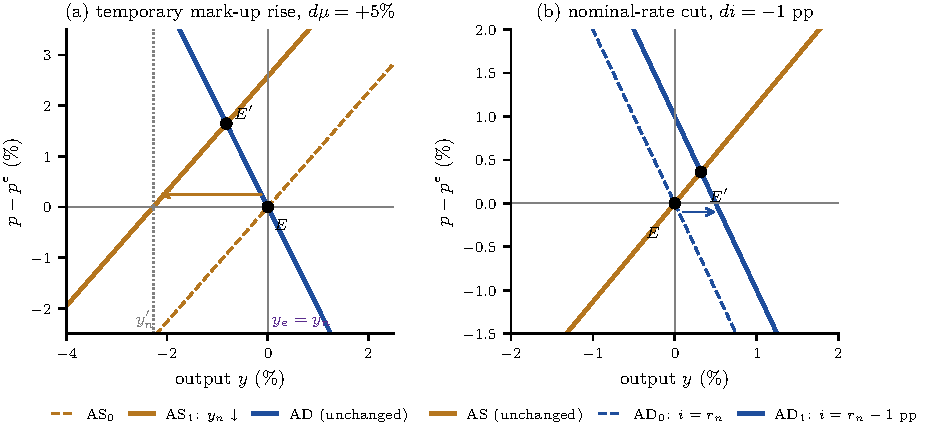
\includegraphics[width=0.94\textwidth]{fig/fig_l7q2_shocks.pdf}\\[2pt]
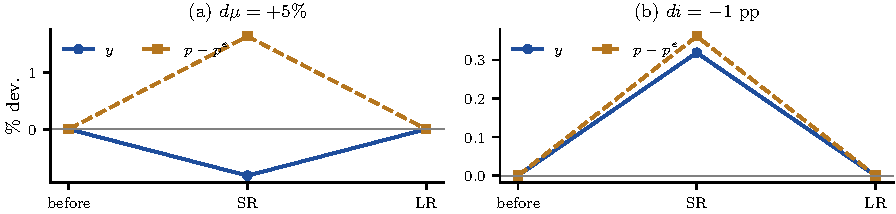
\includegraphics[width=0.94\textwidth]{fig/fig_l7q2_paths.pdf}
\end{minipage}
\end{center}

%=====================================================================
\q{3} $y_n$ vs $y_e$

\begin{itemize}
\item $y_n$: flexible prices, \emph{decentralised} economy (market power and taxes kept)
      $\ra$ AS anchor; $y-y_n$ drives \textbf{prices}.
\item $y_e$: \emph{planner}, $\max u(C)-v(L)$ s.t.\ $Y=C+G$, $Y=AL$; $y-y_e$ drives
      \textbf{welfare}. Neither depends on $\alpha$.
\end{itemize}

\emph{Planner.} Substitute both constraints: $\max_Y\,u(Y-G)-v(Y/A)$
$\ra u_c(Y-G)-\tfrac1A v_l(Y/A)=0\ra\dfrac{v_l}{u_c}=A$ \;($\MRS=\MRT$).

\emph{Market.} Every firm resets: $P=(1+\mu)\dfrac WA\ra\dfrac WP=\dfrac A{1+\mu}$; household
$\dfrac{v_l}{u_c}=\dfrac WP\ra\dfrac{v_l}{u_c}=\dfrac{A}{\underbrace{1+\mu}_{\text{wedge}}}$.

\emph{Logs.} $v_l=L^\eta$, $L=Y/A\ra\ln v_l=\eta(y-a)$; $u_c=C^{-\tilde\sigma^{-1}}$,
$c=\tfrac{y-g}{s_c}$, $\tilde\sigma^{-1}=s_c\sigma^{-1}\ra\ln u_c=-\sigma^{-1}(y-g)$
$\ra\ln\tfrac{v_l}{u_c}=\eta(y-a)+\sigma^{-1}(y-g)$.
\begin{align*}
\text{planner: }&\eta(y_e-a)+\sigma^{-1}(y_e-g)=a
  &&\ra\;\Sg y_e=(1+\eta)a+\sigma^{-1}g\\
\text{market: }&\eta(y_n-a)+\sigma^{-1}(y_n-g)=a-\mu
  &&\ra\;\Sg y_n=(1+\eta)a+\sigma^{-1}g-\mu
\end{align*}
Subtract: $\Sg(y_n-y_e)=-\mu\ra$
\[
\res{y_n-y_e=-\frac{\mu}{\sigma^{-1}+\eta}}\qquad \mu=5\%:\;-\tfrac{5}{2{,}2}=-2{,}27\%
\]

\emph{Why they differ.} $P>MC\ra W/P=A/(1+\mu)<A=MPL\ra$ household stops at $\MRS=A/(1+\mu)$
$\ra L$, $Y$ too low. Lost surplus = triangle between $\MRT=a$ and $\ln\MRS$ from $y_n$ to $y_e$:
height $\mu$ (gap at $y_n$), base $y_e-y_n=\tfrac{\mu}{\sigma^{-1}+\eta}$
$\ra\tfrac12\mu\cdot\tfrac{\mu}{\sigma^{-1}+\eta}=\tfrac12\tfrac{\mu^2}{\sigma^{-1}+\eta}
=\tfrac12\cdot\tfrac{0{,}05^2}{2{,}2}=0{,}057\%$ of output. Quadratic $\ra$ loss in $(y-y_e)^2$.

\emph{Why a temporary $\mu\uparrow$ moves only $y_n$.}
$y_n=y_n(a,g,\mu)$, $y_e=y_e(a,g)$: the planner's problem has no prices, market power or taxes
\[
\res{dy_n=-\frac{d\mu}{\sigma^{-1}+\eta}<0,\qquad dy_e=0}\ra\text{inefficient shock}\ra\text{trade-off}
\]
Contrast $a\uparrow$: enters both $\ra dy_n=dy_e=\tfrac{1+\eta}{\sigma^{-1}+\eta}da=\tfrac{1{,}2}{2{,}2}\cdot2=1{,}09\%$
for $da=2\%$ (no trade-off).
\nota{$\alpha$ appears in neither: stickiness explains $y\neq y_n$, not $y_n\neq y_e$.}

\begin{center}
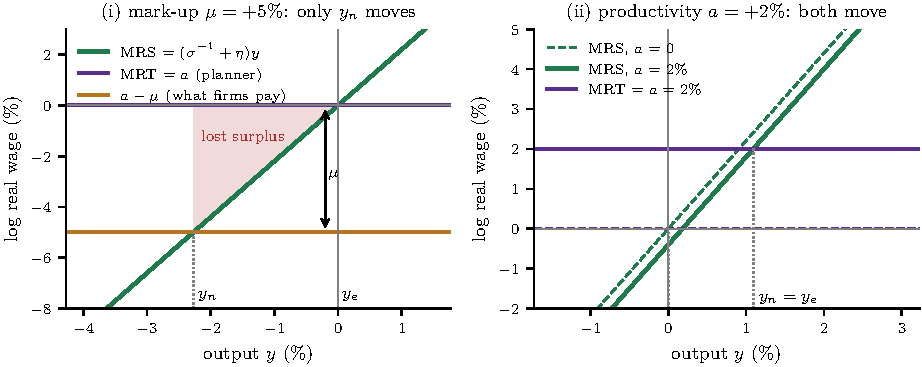
\includegraphics[width=0.9\textwidth]{fig/fig_l7q3_wedge.pdf}
\end{center}

%=====================================================================
\q{4} $\min\;\mathcal L=\phi_y(y-y^*)^2+\phi_p(p-p^e)^2$ s.t.\ $p-p^e=\kappa(y-y_n)$

\textbf{Shape.} $\mathcal L\ge0$, $=0$ only at the bliss point $(y^*,p^e)$. Quadratic $\ra$
symmetric (booms as bad as recessions: the CB \emph{stabilises}) and convex
($\partial\mathcal L/\partial y=2\phi_y(y-y^*)$ is $0$ at the target and grows with the miss)\\
$\ra$ \rest{spread the miss across both targets}. Iso-loss $\phi_y(y-y^*)^2+\phi_p(p-p^e)^2=\bar{\mathcal L}$:
ellipses, axes $\propto(1/\sqrt{\phi_y},1/\sqrt{\phi_p})$. $\phi_p/\phi_y$ = conservatism (hawk vs dove).
Only surprises cost (dispersion). Welfare version: $\phi_y=\tfrac12$, $\phi_p=\tfrac{\theta}{2\kappa}$, $y^*=y_e$ (eq.~33).

\textbf{Why subject to AS.} One instrument $i$, and $i$ appears only in AD $\ra$ moving $i$ slides
AD \emph{along} AS $\ra$ every point of AS is reachable, no other point is
$\ra$ \rest{AS = feasible set (``budget line'')}, slope $\kappa$ = price of output in surprises.
AD is not a constraint: for any $(y,p)$ on AS there is an $i$ putting AD through it.

\textbf{Solve} (substitute the constraint, no Lagrangian):
\begin{align*}
\mathcal L(y)&=\phi_y(y-y^*)^2+\phi_p\kappa^2(y-y_n)^2\\
\mathcal L'(y)&=2\phi_y(y-y^*)+2\phi_p\kappa^2(y-y_n)=0
  \qquad\mathcal L''(y)=2(\phi_y+\phi_p\kappa^2)>0\;\text{(minimum)}
\end{align*}
Divide by 2, write $\kappa(y-y_n)=p-p^e$:
\[
\res{\phi_y(y-y^*)+\kappa\,\phi_p(p-p^e)=0}\quad\text{(targeting rule)}
\]
Solve $\mathcal L'=0$ for $y$: $(\phi_y+\phi_p\kappa^2)y=\phi_y y^*+\phi_p\kappa^2y_n$. Let $D\equiv\phi_y+\phi_p\kappa^2$, $\Delta\equiv y^*-y_n$:
\begin{align*}
y^o&=\frac{\phi_y y^*+\phi_p\kappa^2y_n}{D},\qquad
y^o-y_n=\frac{\phi_y}{D}\Delta,\qquad y^o-y^*=-\frac{\phi_p\kappa^2}{D}\Delta\\
p^o-p^e&=\kappa(y^o-y_n)=\frac{\kappa\phi_y}{D}\Delta\\
\mathcal L^o&=\phi_y\frac{\phi_p^2\kappa^4}{D^2}\Delta^2+\phi_p\kappa^2\frac{\phi_y^2}{D^2}\Delta^2
=\frac{\phi_y\phi_p\kappa^2(\phi_p\kappa^2+\phi_y)}{D^2}\Delta^2
=\res{\frac{\phi_y\phi_p\kappa^2}{\phi_y+\phi_p\kappa^2}(y^*-y_n)^2}
\end{align*}
Share into prices, relative to strict output ($p-p^e=\kappa\Delta$):
$\dfrac{p^o-p^e}{\kappa\Delta}=\dfrac{\phi_y}{D}$.
Welfare weights: $\phi_p\kappa^2=\tfrac{\theta}{2\kappa}\kappa^2=\tfrac{\theta\kappa}{2}$
$\ra\dfrac{\phi_y}{D}=\dfrac{1/2}{1/2+\theta\kappa/2}=\res{\dfrac{1}{1+\theta\kappa}}$; rule
$\tfrac12(y-y_e)+\kappa\tfrac{\theta}{2\kappa}(p-p^e)=0\ra(y-y_e)+\theta(p-p^e)=0$ (eq.~34).

\textbf{Implementing rate.} From the closed form of Q2:
$y^o-y_n=\tfrac{\sigma}{1+\sigma\kappa}(r_n-i^o)\ra i^o=r_n-\tfrac{1+\sigma\kappa}{\sigma}(y^o-y_n)$.

\emph{Numbers}, $d\mu=5\%$, welfare weights, $y^*=y_e=0$:
\begin{itemize}
\item $\Delta=0-(-2{,}273)=2{,}273$;\quad $\theta\kappa=8\cdot1{,}133=9{,}07$;\quad
      share $=1/10{,}07=0{,}099$
\item $y^o-y_n=0{,}099\cdot2{,}273=0{,}226\ra y^o=-2{,}273+0{,}226=-2{,}05\%$;\quad
      $p^o-p^e=1{,}133\cdot0{,}226=+0{,}26\%$
\item $\phi_p=\tfrac{8}{2\cdot1{,}133}=3{,}53$, $\phi_p\kappa^2=4{,}53$, $D=5{,}03$
      $\ra\mathcal L^o=\tfrac{0{,}5\cdot4{,}53}{5{,}03}\cdot2{,}273^2=0{,}450\cdot5{,}17=2{,}33$
\item $i^o=6{,}55-\tfrac{1{,}567}{0{,}5}\cdot0{,}226=6{,}55-0{,}71=5{,}84\%$
      (vs $2\%$ doing nothing; vs $r_n=6{,}55\%$ for strict price stability)
\item Strict output ($y=0$): $p-p^e=1{,}133\cdot2{,}273=2{,}58\%$,
      $i=6{,}55-3{,}13\cdot2{,}273=-0{,}58\%$ (a cut; zero bound ignored)
\end{itemize}

\textbf{Sign of the response} (vs doing nothing, $i=\rho$; with $y^*=y_e=0$, so
$r_n-\rho=-y_n/\sigma=\Delta/\sigma$). $i^o>\rho\iff
\tfrac{1+\sigma\kappa}{\sigma}\tfrac{\phi_y}{D}\Delta<r_n-\rho=\tfrac{\Delta}{\sigma}
\iff\phi_y(1+\sigma\kappa)<\phi_y+\phi_p\kappa^2\iff\underbrace{\tfrac{\phi_y}{\phi_p\kappa}}_{|\text{IT slope}|}<\underbrace{\tfrac1\sigma}_{|\text{AD slope}|}$.
Welfare: $\tfrac{\phi_y}{\phi_p\kappa}=\tfrac1\theta=0{,}125<2$ $\ra$ raise.
\rest{IT flatter than AD $\ra$ raise $i$; steeper $\ra$ cut}: the sign is a property of the mandate.

\textbf{Policy meaning.}
\begin{itemize}
\item $\Delta=0$ ($a$, $g$ shocks move $y_n=y_e$ together) $\ra y^o=y^*$, $p^o=p^e$,
      $\mathcal L^o=0$, $i=r_n$: divine coincidence.
\item $\Delta\neq0$ ($\mu$ shocks) $\ra\mathcal L^o>0$: trade-off, split $\tfrac{\phi_y}{D}$ into prices.
\item CB picks a point \emph{on} AS, cannot move AS $\ra$ cannot change $y_n-y_e$
      $\ra$ taxes / competition policy.
\item Trade-off only SR and only with sticky prices: $\alpha\to0\ra\kappa\to\infty\ra
      \tfrac{\phi_y}{D}\to0\ra y^o\to y_n$, $p^o\to p^e$. Can't hold $y>y_n$ every period:
      with rational $p^e$, $E[p-p^e]=0\ra E[y-y_n]=0$ (Kydland--Prescott).
\end{itemize}
\nota{AS is the constraint, not AD. $\kappa$ is private pricing technology, not a policy choice.}

\begin{center}
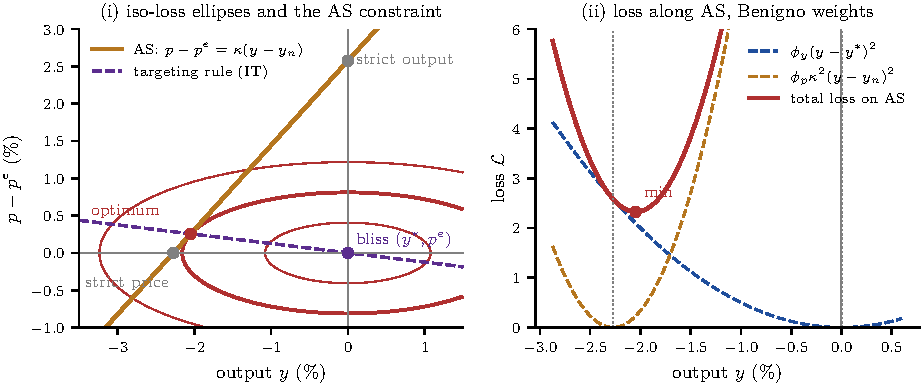
\includegraphics[width=0.9\textwidth]{fig/fig_l7q4_loss.pdf}
\end{center}

\end{document}
